\subsubsection{Scheduling per consolidamento energetico con vincoli di deadline}
\label{subsubsec:e2fis_consolidation}

Accanto agli approcci orientati al bilanciamento della disponibilità
energetica dei nodi, la letteratura propone strategie che perseguono
l'efficienza energetica attraverso il \emph{workload consolidation}.
In questo modello, lo scheduler non mira a distribuire uniformemente
il carico tra i nodi disponibili, bensì a concentrarlo su un
sottoinsieme selezionato, riducendo il numero di elementi attivi e,
di conseguenza, il consumo energetico complessivo dell'infrastruttura.

Un esempio rappresentativo di questo paradigma è E$^{2}$FIS
(\emph{Energy-Efficient Function Invocation Scheduling})~\cite{e2fis_smartcomp},
proposto per piattaforme FaaS nell'edge--cloud continuum. Come
illustrato in Figura~\ref{fig:e2fis_architecture}, il sistema assume
un insieme di nodi eterogenei, ciascuno caratterizzato da capacità
computazionale, memoria disponibile, throughput effettivo e profilo
di consumo energetico. Le funzioni sono descritte tramite requisiti
di memoria, carico computazionale e deadline di completamento; la
stima del tempo di esecuzione tiene conto delle differenze
architetturali tra nodi, consentendo di verificare la compatibilità
di ciascuna assegnazione con i vincoli temporali imposti.

\begin{figure}[ht]
    \centering
    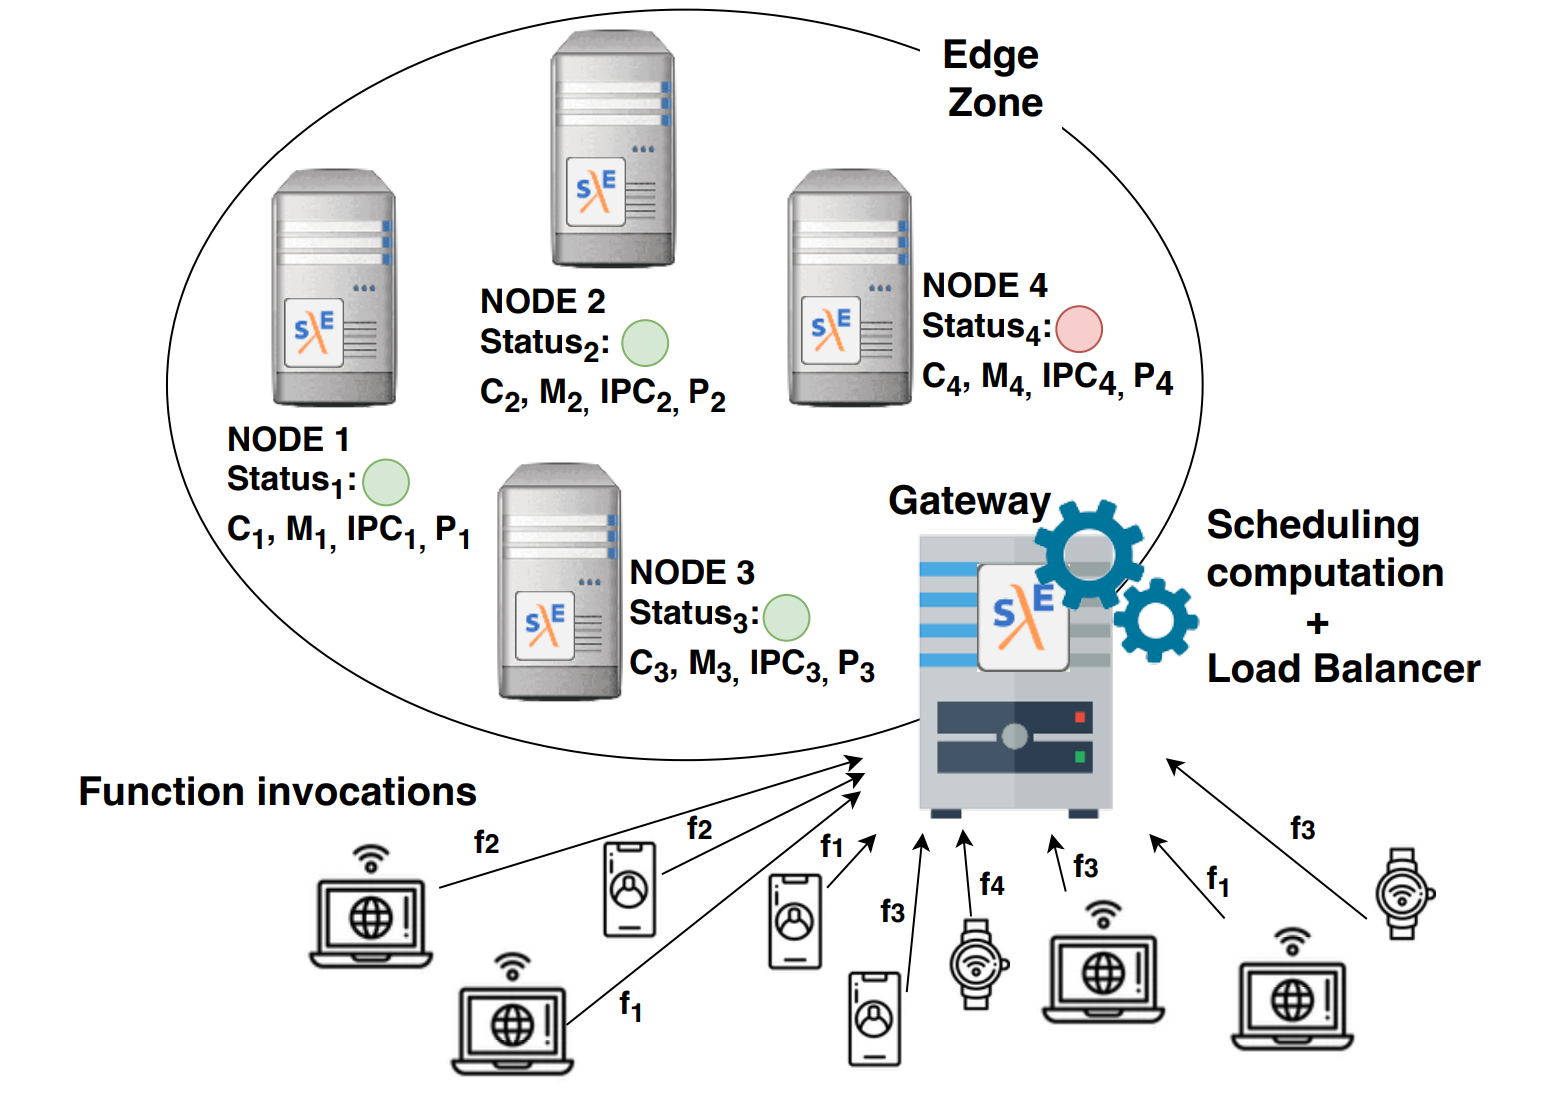
\includegraphics[width=0.85\textwidth]{figures/EnergyEfficientFunctionArchitecture.png}
    \caption{Architettura di E$^{2}$FIS. I nodi edge sono caratterizzati
    da differenti capacità computazionali e profili di consumo. Il modulo
    di \emph{Scheduling computation} determina periodicamente l'allocazione
    delle funzioni e il sottoinsieme di nodi da mantenere attivi.}
    \label{fig:e2fis_architecture}
\end{figure}

L'approccio adotta una pianificazione periodica basata su epoche
temporali discrete. Prima dell'inizio di ciascuna epoca, il problema
di allocazione viene formulato come un'istanza di Programmazione
Lineare Intera Mista (MILP) e risolto offline. La funzione obiettivo
minimizza il consumo energetico associato ai nodi attivi
nell'intervallo considerato, selezionando il sottoinsieme minimo
necessario a soddisfare tutte le richieste entro le rispettive
deadline. Ne deriva una logica di consolidamento: quando il carico
complessivo lo consente, le invocazioni vengono concentrate sui nodi
con il miglior rapporto tra capacità computazionale e consumo
energetico, mentre i restanti possono essere portati in stato inattivo.

Per garantire robustezza operativa in presenza di istanze
computazionalmente onerose, il sistema prevede un limite temporale
per la risoluzione del problema di ottimizzazione: qualora la
soluzione ottima non sia ottenibile entro la soglia stabilita, viene
adottata la migliore soluzione ammissibile disponibile. In scenari di
carico elevato o con vincoli particolarmente stringenti, il framework
può inoltre ricorrere a una politica di fallback ispirata a EDF
(\emph{Earliest Deadline First}), privilegiando il rispetto delle
deadline rispetto all'ottimizzazione energetica.
Tale meccanismo evidenzia come, in condizioni limite, il rispetto dei
vincoli temporali costituisca un obiettivo prioritario rispetto
all'efficienza energetica, introducendo una gerarchia esplicita tra
gli obiettivi del sistema.

Nel complesso, E$^{2}$FIS rappresenta un approccio di scheduling
energeticamente consapevole a granularità di nodo, nel quale il
consumo energetico è trattato come metrica di ottimizzazione piuttosto
che come vincolo fisico esplicito. L'adattamento si realizza
esclusivamente attraverso la selezione del sottoinsieme di nodi attivi
e l'assegnazione delle invocazioni, senza intervenire sulla logica
applicativa né prevedere varianti delle funzioni con profili energetici
differenziati. Analogamente a Faashouse, il perimetro decisionale
rimane quindi circoscritto al livello infrastrutturale, lasciando
inesplorata la possibilità di modulare il consumo energetico agendo
direttamente sull'implementazione delle funzioni invocate.